\setcounter{chapter}{0}
\chapter{Giới thiệu bài toán}
Với sự tiến bộ nhanh chóng trong công nghệ thương mại điện tử, việc sử dụng thẻ tín dụng để phục vụ nhu cầu trong đời sống cũng như trong doanh nghiệp đã tăng lên một cách đáng kể. Ngày nay, thẻ tín dụng đang trở thành phương thức thanh toán phổ viến nhất trong việc mua hàng trực tuyến, cũng như mua hàng trực tiếp, bởi vậy mà các trường hợp gian lận thẻ tín dụng cũng đang gia tăng. Trong bài báo cáo này, nhóm chúng em sử dụng mô hình Makov ẩn (Hiden Makov Model – HMM) để nghiên cứu, mô hình hóa chuỗi hoạt động trong việc xử lý thông tin giao dịch thẻ tín dụng và chỉ ra cách phát hiện gian lận.
\section{Thẻ tín dụng}
Chiếc thẻ ngân hàng đầu tiên được xuất hiện từ năm 1946 với cái tên "Chard-lt", do John Biggins ở Brooklyn nghĩ ra. Khi khách hàng mua sắm, hóa đơn được chuyển đến ngân hàng của Biggins. Ngân hàng trả tiền cho người bán và sau đó khách hàng trả tiền cho ngân hàng. Điểm trừ là loại thẻ nay chỉ sử dụng trong phạm vi địa phương và dành riêng cho khách của ngân hàng. Năm 1949, sau một lần đi ăn nhà hàng gặp vấn đề về việc thanh toán, người đàn ông tên Frank McNamara cùng với đối tác đã lập ra công ty Diners Club, phát hành loại thẻ chuyên dùng để thanh toán tại các nhà hàng – tiền thân của thẻ tín dụng hiện nay. Từ đó, thẻ tín dụng đã và đang trở thành một loại thẻ vô cùng cần thiết trong cuộc sống hiện nay, đáp ứng mọi nhu cầu về việc thanh toán nhanh và tiện lợi. 

Để nghiên cứu sâu hơn các vấn đề liên quan đến thẻ tín dụng, đặc biệt là việc phát hiện gian lận thẻ tín dụng chúng ta cần hiểu rõ: "Thẻ tín dụng (Credit Card) là gì?" và "Lợi ích của thẻ tín dụng".

Thẻ tín dụng là một loại thẻ ngân hàng mà người sở hữu có thể dùng để thanh toán mà không cần tiền có sẵn trong thẻ. Điều này có nghĩa là bạn "mượn" một số tiền của ngân hàng để mua sắm, chi tiêu và cuối kì sẽ phải trả lại đầy đủ cho ngân hàng. Những tiện ích khi sử dụng đã chứng minh thẻ tín dụng là công cụ hữu ích nhất trong thanh toán và giao dịch. Ngày nay, người tiêu dùng thường thích mang thẻ tín dụng hơn tiền mặt vì những lý do sau đây:
\begin{itemize}
	\item Công cụ hỗ trợ tài chính.
	\item Thanh toán tiện lợi
	\item Quản lý chi tiêu
	\item Nhận được nhiều ưu đãi (Các chương trình giảm giá, chiết khấu khi đặt dịch vụ)
	\item ...
\end{itemize}

\section{Gian lận thẻ tín dụng}
Gian lận là một trong những vấn đề được quan tâm chính trong ngành tín dụng. Thẻ tín dụng là một trong những mục tiêu lừa đảo nổi tiếng vì sự phổ biến cùng với những tiện ích mà nó mang lại cho người tiêu dùng. Gian lận thẻ tín dụng là hình thức gian lận sử dụng công nghệ cao để đánh cắp thông tin thẻ tín dụng (Visa, MasterCard, ATM,...) của người sử dụng, thuộc về lĩnh vực tài chính, ngân hàng. 

\begin{center}
	
	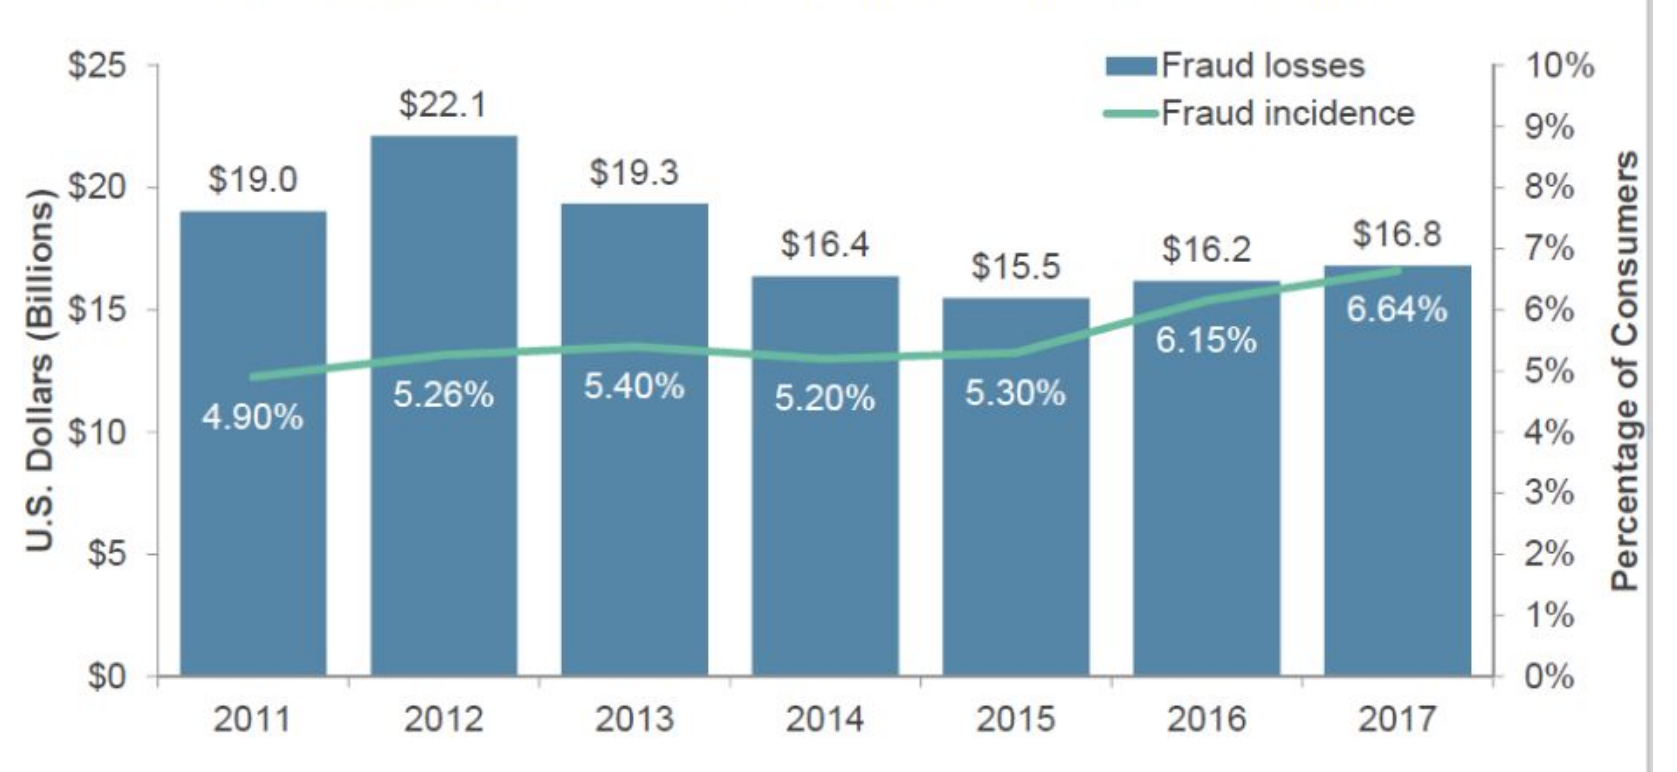
\includegraphics[scale=0.3]{11.png}
	
	
	\textit{Hình 1.1:} Tỉ lệ lừa đảo và số lượng tiền đã mất do gian giận thẻ tí dụng, 2011-2017 \footnote{Javelin Strategy \& Research 2018}
\end{center}


Một số hình thức gian lận thẻ tín dụng:
\begin{itemize}
	\item Bị thanh toán hay quẹt thẻ tại một cửa hàng nào đó khi mua hàng trong trường hợp bạn bị trộm thẻ.
	\item Sử dụng công nghệ cao qua mạng Internet đánh cắp thông tin thẻ tín dụng của người dùng.
	\item Bị rút tiền mặt qua máy ATM.
	\item Làm giả thẻ Visa, MasterCard.
	\item ...
\end{itemize}

\section{Bài toán}
Bài toán "phát hiện gian lận thẻ tín dụng" đã thu hút rất nhiều sự quan tâm nghiên cứu, một kỹ thuật đặc biệt mà một số nghiên cứu sử dụng là chú trọng vào khai thác dữ liệu và mạng neural. Trên thực tế, đã có một số cách tiếp cận để xử lý bài toán trên dựa trên tiêu chuẩn của dữ liệu trong các giao dịch chính hãng, so sánh chúng trong các trường hợp giao dịch gian lận, từ đó để phân loại các kiểu gian lận, làm tiêu chuẩn để phát hiện gian lận. Nhưng việc lấy dữ liệu các giao dịch gian lận trong thực tế là một trong những vấn đề khó khăn. Ngoài ra những phương pháp đó không thể phát hiện được các kiểu gian lận mới mà dữ liệu được dán nhãn không có sẵn. Trong bài báo cáo này, nhóm trình bày phương pháp phát hiện gian lận thẻ tín dụng dựa trên mô hình Markov ẩn (HMM). Nhóm mô hình hóa thông tin giao dịch thẻ tín dụng theo mô hình Markov ẩn. Các giao dịch chỉ có thể được quan sát thông qua quy trình ngẫu nhiên tạo ra chuỗi bao gồm số tiền thanh toán, loại hàng hóa thanh toán,... trong mỗi giao dịch. Do đó, HMM là một lựa chọn lý tưởng để giải quyết bài toán này.





